\section{Method}

\begin{frame}
    \frametitle{Problem Statement}

    \begin{itemize}
        \item Agent searches scene \(S \subset \mathbb{R}^d\) .
        \item Scene contains set of targets \(\{t_0, \dots t_n\}\), \(t_i \in S\).
        \item Agent perceives view \(V \subset S\).
        \item Move actions transform view to new subspace.
        \item Final action indicates that a target is in view.
        \item Select actions that maximize the probability of finding all targets while minimizing cost in time.
        \item NP complete~\cite{andreopoulos_theory_2009}, intractable to solve optimally.
    \end{itemize}
\end{frame}

\subsection{Environments}

\begin{frame}
    \frametitle{Environments}
    
    \begin{itemize}
        \item Three simulated environments used for experiments.
        \item Search space discretized into \(10 \times 10\) camera positions.
        \item Each camera position has a unique view \(V \subset S\).
        \item Three targets in all scenes.
        \item Target probability correlated with scene appearance.
        \item Should be possible to do better than exhaustive search on average.
        \item Scenes procedurally generated:
        \begin{itemize}
            \item Pseudorandom seed determines scene appearance and target positions.
            \item Gives control over difficulty to solve.
            \item Can vary training and test set sizes.
        \end{itemize}
    \end{itemize}
\end{frame}

\begin{frame}
    \frametitle{Observation, Action and Reward}

    At each time step \(t\):

    \begin{itemize}
        \item The agent receives observation \(o_t = \left\langle x_t, p_t \right\rangle\), where
        \begin{itemize}
            \item \(x_t \in \mathbb{R}^{3 \times 64 \times 64}\) is an RGB image of current view, and
            \item \(p_t \in \{0, \dots, 9\} \times \{0, \dots, 9\}\) is the position of the camera.
        \end{itemize}
        \item Takes action \(a_t \in \{\texttt{INDICATE}, \texttt{UP}, \texttt{DOWN}, \texttt{LEFT}, \texttt{RIGHT}\}\), where
        \begin{itemize}
            \item \texttt{INDICATE} indicates that a target is in view, and
            \item \texttt{UP}, \texttt{DOWN}, \texttt{LEFT}, \texttt{RIGHT} move the view in each cardinal direction.
        \end{itemize}
        \item Receives reward \(r_t = h - 0.01 + 0.005d + 0.005e\) where
        \begin{itemize}
            \item \(h = \left\vert T \cap V \right\vert\) if \(a_t = \texttt{INDICATE}\).
            \item \(d = 1\) if \(a_t\) moves closer to nearest target.
            \item \(e = 1\) if \(a_t\) moves to new position.
            \item Rewarded for finding targets, moving towards them and exploring environment.
            \item Constant penalty encourages quick episode completion.
        \end{itemize}
    \end{itemize}
\end{frame}

\begin{frame}
    \frametitle{Environment I: Gaussian}
    \begin{columns}
        \begin{column}{0.5\textwidth}
            \begin{itemize}
                \item 2D scene.
                \item Three gaussian kernels with random center.
                \item Sum of kernels determine appearance of scene and probability of targets.
                \item Clear correlation between appearance and desired behavior.
            \end{itemize}
        \end{column}
        \begin{column}{0.5\textwidth}
            \begin{figure}
                \centering
                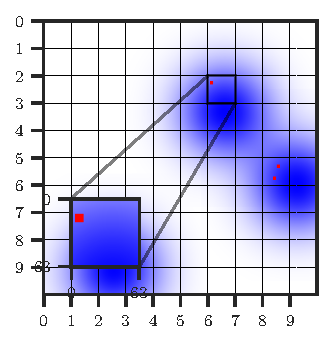
\includegraphics[scale=1.0]{figures/gaussian.pdf}
            \end{figure}
        \end{column}
    \end{columns}    
\end{frame}

\begin{frame}
    \frametitle{Environment II: Terrain}
    \begin{columns}
        \begin{column}{0.5\textwidth}
            \begin{itemize}
                \item Similar to previous environment.
                \item Terrain seen from above.
                \item Gradient noise used to generate height map.
                \item Color determined by height.
                \item Targets placed with uniform probability across coastlines.
                \item More realistic, higher variance.
                \item Analogous to search and rescue with UAV.
            \end{itemize}
        \end{column}
        \begin{column}{0.5\textwidth}
            \begin{figure}
                \centering
                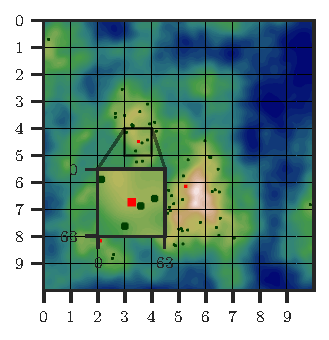
\includegraphics[scale=1.0]{figures/terrain.pdf}
            \end{figure}
        \end{column}
    \end{columns}   
\end{frame}

\begin{frame}
    \frametitle{Environment III: Camera}
    \begin{columns}
        \begin{column}{0.5\textwidth}
            \begin{itemize}
                \item 3D scene viewed from a perspective projection camera.
                \item Height map from terrain environment turned into mesh, same appearance and target probability as before.
                \item Camera location fixed at center of scene.
                \item Moving actions control pan and tilt (pitch and yaw).
                \item Visually complex, difficult to interpret.
            \end{itemize}
        \end{column}
        \begin{column}{0.5\textwidth}
            \begin{figure}
                \centering
                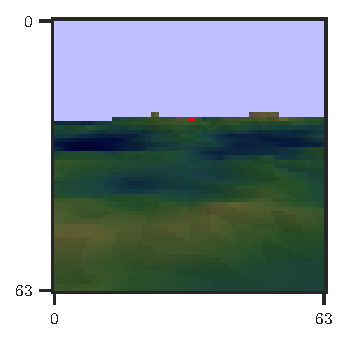
\includegraphics[scale=1.0]{figures/camera.pdf}
            \end{figure}
        \end{column}
    \end{columns}
\end{frame}

\subsection{Approach}

\begin{frame}
    \frametitle{Approach}
\end{frame}

\begin{frame}
    \frametitle{Architecture}

    \begin{itemize}
        \item Actor-critic method trained with PPO~\cite{schulman_proximal_2017}.
        \item Image \(x_t\) passed through CNN.
        \item Latent image representation \(y_t\) and position \(p_t\) passed through RNN with recurrent state \(z_t\).
        \item Policy and value heads approximate \(\pi\) and \(v_\pi\) from \(h_t\) with MLPs.
    \end{itemize}

    \begin{figure}
        \centering
        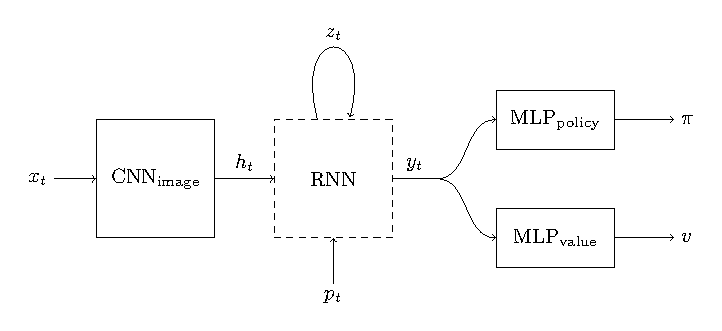
\includegraphics[scale=0.7]{figures/architecture.pdf}
    \end{figure}
\end{frame}

\begin{frame}
    \frametitle{Memory}

    \begin{itemize}
        \item Recurrent step serves as memory.
        \item Necessary to remember features of explored environment.
        \item Two variants evaluated:
        \begin{enumerate}
            \item Temporal memory (LSTM)
            \item Spatial memory.
        \end{enumerate}
    \end{itemize}
\end{frame}

\begin{frame}
    \begin{enumerate}
        \item LSTM:
        \begin{itemize}
            \item Proven to work for POMDPs \cite{hausknecht_deep_2017,mnih_asynchronous_2016,mirowski_learning_2017,gupta_cognitive_2019}.
            \item May struggle with remembering over many time steps.
            \item Important for exhaustive search and scene understanding.
        \end{itemize}
        \item Spatial memory (inspired by \cite{parisotto_neural_2017}):
        \begin{itemize}
            \item Structured memory \(M_t \in \mathbb{R}^{C \times 10 \times 10}\) as hidden state \\
            (one slot per camera position \(p_t\) / unique view \(V\) / image \(x_t\)).
            \item Read vector \(r_t = f(M_t)\), \(f\) is CNN.
            \item Write vector \(w_t = g(\left\lbrack h_t, r_t \right\rbrack)\), \(g\) is MLP.
            \item Action probabilities \(\pi(\left\lbrack r_t, w_t \right\rbrack)\) and value \(v(\left\lbrack r_t, w_t \right\rbrack)\).
            \item \(r_t\) contains information from the whole explored scene.
            \item \(w_t\) written to index \(p_t\) of \(M_{t+1}\).
        \end{itemize}
    \end{enumerate}
\end{frame}

\begin{frame}
    \frametitle{Experiments}

    \begin{enumerate}
        \item Search Performance
        \item Scaling to Larger Search Spaces
        \item Generalization from Limited Samples
    \end{enumerate}

    \begin{itemize}
        \item Train for 25M time steps.
        \item Results reported across 3 runs with different seeds.
        \item Separate training and test sets.
        \item Same hyperparameters in all runs.
    \end{itemize}
\end{frame}


\begin{frame}
    \frametitle{Implementation}

    \begin{itemize}
        \item OpenAI Gym environment interface.
        \item PyTorch for models and automatic differentiation.
        \item Intel Core i9-10900X CPU.
        \item NVIDIA GeForce RTX 2080 Ti GPU.
    \end{itemize}
\end{frame}